\documentclass{article}
\usepackage[utf8]{inputenc}
\usepackage[a4paper, total={6.4in, 8.53in}]{geometry}
\usepackage{amsmath, tikz, amsfonts, bbm, mathrsfs, graphicx, amssymb, amsthm, hyperref, centernot, enumerate, bbm, xcolor, lmodern, mathdots, amsfonts, graphicx,float}
\graphicspath{ {./output/} }

\title{MAT1856/APM466 Assignment 1}
\author{Yiqu Ding, Student \#: 1004913329}
\date{February, 2022}

\begin{document}

\maketitle

\section*{Fundamental Questions - 25 points}

\begin{enumerate}
    \item \hfill
    \begin{enumerate}
        \item Governments issue bonds and not simply print more money because they want to control the total money supply and not to inflation.
        \item Suppose the bank plan to increase interest rates recently to attarct client deposits, this will cause the yield to rise in a short period, but it is almost certain that as time goes by, the bank has had enough increased deposits and decide to decrease the rate again and the long-term yield curve will increase less rapidly.
        \item Quantitative easing is a monetary policy that the US Fed used during the COVID-19 Pandemic. They purchased long-term bonds from banks across the US to increase their money supply and lower the interest rate(risk-free rate) to stimulate the investment market and thus boosting the economy. 
    \end{enumerate}
    \item  I am picking 10 coupons with the first one maturing in less than 6 months, the second one maturing at least 6 months later but sooner than 1 year, the third one matures in at least a year but less than 1 year plus 6 months, etc. This way my first bond will have 1 payment left, the second one has 2 payments left and etc. I can treat my first bond(maturing in less than 6 months) as a zero coupon bond because it has no coupon payment left, and use this to calculate the yield of the first coupon, then I go on and treat the second half of my second bond as a zero coupon again, I continue this process in order to get my 5 year curve.
    \item The eigenvalues and eigenvectors of the covariance matrix of stoghastic processes are called principle components. Just like how its name suggests, the principle components of the covariance matrix contains the most information carried in the model built, in other words we can obtain the most inportant results from a very complex model by only viewing its principle components. The first eigenvector indicates the correlation between curves, it captures the curve dynamics. The second eigenvector represents the steepening of the curve and the third vector represents the level of change in convexity. After that it is mainly noise.
\end{enumerate}


\section*{Empirical Questions - 75 points} 

\begin{enumerate}
\setcounter{enumi}{3} 
    \item Please see the reference for the source of codes.
    \begin{enumerate}
        \item Please see \ref{4a} for the plot of the yield curve.
        \item Please see \ref{4b} for the plot of the spots curve.
            \begin{figure}
            \centerline{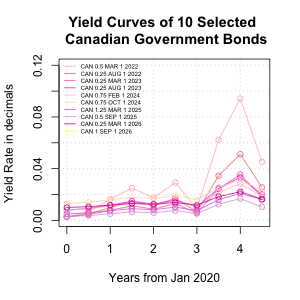
\includegraphics{YTM.png}}
            \caption{Q4(a)}
            \label{4a}
            \centerline{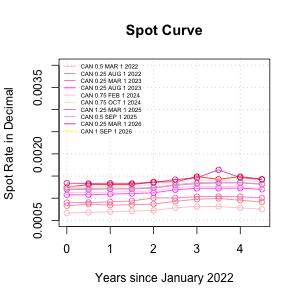
\includegraphics{SPOT.png}}
            \caption{Q4(b)}
            \label{4b}
            \centerline{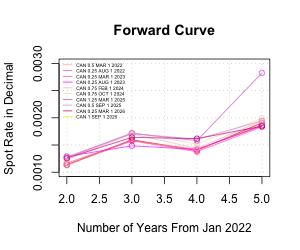
\includegraphics{Forward.png}}
            \end{figure}
        \item Please see \ref{4c} for the plot of the forward curve. 
            \begin{figure}[hbt!]
            \caption{Q4(c)}
            \label{4c}
            \end{figure}
    \end{enumerate}
    \item Please see \ref{5} and \ref{6}.
    \item Please see \ref{Eigens} for the eigenvectors. The corresponing eigen values are
    (1.646460,2.716362e-02,1.530982e-03,5.252046e-04,5.215349e-05) and 
    (5.446583e-01,3.203774e-02,1.915300e-17,4.276895e-18,3.604313e-18,1.918414e-18,1.353332e-18,4.562149e-19,4.327970e-19,-1.082219e-16).
    We osberve that all entries of the first eigenvevtor are negative, which indicates that the dominant motions of all curves are similiar and are negatively related.
    \begin{table}[ht]
    \centering
    \begin{tabular}{rrrrrr}
    \hline 
 & log\_return1 & log\_return2 & log\_return3 & log\_return4 & log\_return5 \\ 
    \hline
log\_return1 & 0.92 & 0.66 & 0.30 & 0.30 & 0.19 \\ 
  log\_return2 & 0.66 & 0.49 & 0.23 & 0.22 & 0.15 \\ 
  log\_return3 & 0.30 & 0.23 & 0.11 & 0.11 & 0.07 \\ 
  log\_return4 & 0.30 & 0.22 & 0.11 & 0.10 & 0.07 \\ 
  log\_return5 & 0.19 & 0.15 & 0.07 & 0.07 & 0.05 \\ 
   \hline
    \end{tabular}
    \caption{Log Return Covariance Matrix}
    \label{5}
    \end{table}

    \begin{table}[ht]
    \centering
    \begin{tabular}{rrrrrrrrrrr}
    \hline
& fwd1 & fwd2 & fwd3 & fwd4 & fwd5 & fwd6 & fwd7 & fwd8 & fwd9 & fwd10 \\ 
    \hline
fwd1 & 0.07 & 0.06 & 0.06 & 0.07 & 0.04 & 0.07 & 0.07 & 0.08 & 0.05 & 0.03 \\ 
  fwd2 & 0.06 & 0.06 & 0.06 & 0.06 & 0.03 & 0.07 & 0.06 & 0.07 & 0.04 & 0.03 \\ 
  fwd3 & 0.06 & 0.06 & 0.06 & 0.06 & 0.03 & 0.07 & 0.06 & 0.07 & 0.04 & 0.03 \\ 
  fwd4 & 0.07 & 0.06 & 0.06 & 0.06 & 0.04 & 0.07 & 0.06 & 0.07 & 0.04 & 0.03 \\ 
  fwd5 & 0.04 & 0.03 & 0.03 & 0.04 & 0.02 & 0.04 & 0.03 & 0.05 & 0.02 & 0.01 \\ 
  fwd6 & 0.07 & 0.07 & 0.07 & 0.07 & 0.04 & 0.08 & 0.07 & 0.08 & 0.05 & 0.04 \\ 
  fwd7 & 0.07 & 0.06 & 0.06 & 0.06 & 0.03 & 0.07 & 0.06 & 0.07 & 0.04 & 0.03 \\ 
  fwd8 & 0.08 & 0.07 & 0.07 & 0.07 & 0.05 & 0.08 & 0.07 & 0.11 & 0.05 & 0.03 \\ 
  fwd9 & 0.05 & 0.04 & 0.04 & 0.04 & 0.02 & 0.05 & 0.04 & 0.05 & 0.03 & 0.02 \\ 
  fwd10 & 0.03 & 0.03 & 0.03 & 0.03 & 0.01 & 0.04 & 0.03 & 0.03 & 0.02 & 0.02 \\ 
   \hline
\end{tabular}
\caption{Forward Covariance Matrix}
\end{table}
\label{6}

\begin{table}[ht]
\centering
\begin{tabular}{rrrrrr}
  \hline
 & 1 & 2 & 3 & 4 & 5 \\ 
  \hline
1 & 0.74 & 0.59 & 0.20 & -0.24 & -0.03 \\ 
  2 & 0.54 & -0.28 & -0.32 & 0.70 & 0.18 \\ 
  3 & 0.25 & -0.52 & 0.43 & -0.02 & -0.70 \\ 
  4 & 0.25 & -0.34 & -0.66 & -0.62 & -0.04 \\ 
  5 & 0.16 & -0.44 & 0.48 & -0.26 & 0.69 \\ 
   \hline
\end{tabular}
\centering
\begin{tabular}{rrrrrrrrrrr}
  \hline
 & 1 & 2 & 3 & 4 & 5 & 6 & 7 & 8 & 9 & 10 \\ 
  \hline
1 & -0.36 & -0.10 & 0.71 & 0.00 & 0.00 & 0.00 & 0.00 & 0.00 & 0.00 & -0.60 \\ 
  2 & -0.33 & -0.16 & 0.43 & 0.31 & -0.04 & -0.11 & 0.10 & 0.11 & 0.00 & 0.74 \\ 
  3 & -0.32 & -0.19 & -0.04 & -0.54 & -0.25 & 0.43 & -0.20 & -0.14 & -0.48 & 0.17 \\ 
  4 & -0.34 & -0.05 & -0.17 & 0.25 & 0.55 & 0.14 & -0.40 & -0.53 & 0.15 & 0.01 \\ 
  5 & -0.20 & 0.34 & -0.02 & -0.26 & 0.62 & -0.21 & 0.38 & 0.16 & -0.42 & 0.03 \\ 
  6 & -0.38 & -0.09 & -0.30 & 0.15 & -0.08 & 0.46 & 0.65 & 0.04 & 0.27 & -0.11 \\ 
  7 & -0.33 & -0.13 & -0.13 & -0.56 & 0.03 & -0.36 & -0.13 & 0.21 & 0.59 & 0.07 \\ 
  8 & -0.41 & 0.75 & -0.13 & 0.19 & -0.36 & -0.04 & -0.26 & 0.12 & -0.02 & -0.04 \\ 
  9 & -0.24 & -0.27 & -0.28 & 0.14 & -0.30 & -0.62 & 0.19 & -0.38 & -0.30 & -0.14 \\ 
  10 & -0.17 & -0.38 & -0.28 & 0.30 & 0.14 & 0.01 & -0.31 & 0.67 & -0.24 & -0.17 \\ 
   \hline
\end{tabular}
\caption{Eigenvectors for the Yield Cov Matrix and for the Forwards Matrix}
\label{Eigens}
\end{table}

\end{enumerate}

\section*{References and GitHub Link to Code}
    Please refer to \url{https://github.com/dding33/Fixed-Income-Market-Yield-Analysis} for a complete repository containing all data and scripts used for this report. 
    The data used in the analysis was scraped by the author on markets insider at \url{https://markets.businessinsider.com/}.

\end{document}
